%%%%%%%%%%%%%%%%%%%%%%%%%%%%%%%%%%%%%%%%%
% Beamer Presentation
% LaTeX Template
% Version 1.0 (10/11/12)
%
% This template has been downloaded from:
% http://www.LaTeXTemplates.com
%
% License:
% CC BY-NC-SA 3.0 (http://creativecommons.org/licenses/by-nc-sa/3.0/)
%
%%%%%%%%%%%%%%%%%%%%%%%%%%%%%%%%%%%%%%%%%

%----------------------------------------------------------------------------------------
%	PACKAGES AND THEMES
%----------------------------------------------------------------------------------------

\documentclass{beamer}

\mode<presentation> {

% The Beamer class comes with a number of default slide themes
% which change the colors and layouts of slides. Below this is a list
% of all the themes, uncomment each in turn to see what they look like.

%\usetheme{default}
%\usetheme{AnnArbor}
%\usetheme{Antibes}
%\usetheme{Bergen}
%\usetheme{Berkeley}
%\usetheme{Berlin}
%\usetheme{Boadilla}
%\usetheme{CambridgeUS}
%\usetheme{Copenhagen}
%\usetheme{Darmstadt}
%\usetheme{Dresden}
%\usetheme{Frankfurt}
%\usetheme{Goettingen}
%\usetheme{Hannover}
%\usetheme{Ilmenau}
%\usetheme{JuanLesPins}
%\usetheme{Luebeck}
\usetheme{Madrid}
%\usetheme{Malmoe}
%\usetheme{Marburg}
%\usetheme{Montpellier}
%\usetheme{PaloAlto}
%\usetheme{Pittsburgh}
%\usetheme{Rochester}
%\usetheme{Singapore}
%\usetheme{Szeged}
%\usetheme{Warsaw}

% As well as themes, the Beamer class has a number of color themes
% for any slide theme. Uncomment each of these in turn to see how it
% changes the colors of your current slide theme.

%\usecolortheme{albatross}
%\usecolortheme{beaver}
%\usecolortheme{beetle}
%\usecolortheme{crane}
%\usecolortheme{dolphin}
%\usecolortheme{dove}
%\usecolortheme{fly}
%\usecolortheme{lily}
%\usecolortheme{orchid}
%\usecolortheme{rose}
%\usecolortheme{seagull}
%\usecolortheme{seahorse}
\usecolortheme{whale}
%\usecolortheme{wolverine}

\setbeamertemplate{footline} % To remove the footer line in all slides uncomment this line
%\setbeamertemplate{footline}[page number] % To replace the footer line in all slides with a simple slide count uncomment this line

\setbeamertemplate{navigation symbols}{} % To remove the navigation symbols from the bottom of all slides uncomment this line

}

\usepackage{graphicx} % Allows including images
\usepackage{booktabs} % Allows the use of \toprule, \midrule and \bottomrule in tables
\usepackage{sansmathaccent}

\pdfmapfile{+sansmathaccent.map}
\usepackage[plain]{algorithm}
\usepackage{algorithmicx}
\usepackage[noend]{algpseudocode}
\usepackage{listings}
\newcommand{\pseudoli}[1]{\lstinline[style=pseudo]!#1!}
% Deprecated Environments (Replaced by Algorithmic package)
\lstdefinestyle{pseudo}{basicstyle=\rmfamily,
                        upquote=true,
                        keywordstyle=\color{black}\bfseries,
                        commentstyle=\color[rgb]{0.133,0.545,0.133},
                        stringstyle=\color[rgb]{0.627,0.126,0.941},}
                        
\usepackage{tikz}
\usetikzlibrary{trees, arrows, shapes, positioning, decorations}

%----------------------------------------------------------------------------------------
%	TITLE PAGE
%----------------------------------------------------------------------------------------

\title[Search]{Graph Search Algorithms} % The short title appears at the bottom of every slide, the full title is only on the title page

%\author{John Smith} % Your name
\institute[BYU] % Your institution as it will appear on the bottom of every slide, may be shorthand to save space
{
Brigham Young University \\ % Your institution for the title page
\medskip
%\textit{john@smith.com} % Your email address
}
\date{\today} % Date, can be changed to a custom date

\begin{document}

\begin{frame}
\titlepage % Print the title page as the first slide
\end{frame}

%\begin{frame}
%\frametitle{Overview} % Table of contents slide, comment this block out to remove it
%\tableofcontents % Throughout your presentation, if you choose to use \section{} and %\subsection{} commands, these will automatically be printed on this slide as an overview of your presentation
%\end{frame}

%----------------------------------------------------------------------------------------
%	PRESENTATION SLIDES
%----------------------------------------------------------------------------------------

%------------------------------------------------
%\section{First Section} % Sections can be created in order to organize your presentation into %discrete blocks, all sections and subsections are automatically printed in the table of contents %as an overview of the talk
%------------------------------------------------

%\subsection{Subsection Example} % A subsection can be created just before a set of slides with %a common theme to further break down your presentation into chunks

%\begin{frame}
%\frametitle{AVL trees}
%Sed iaculis dapibus gravida. Morbi sed tortor erat, nec interdum arcu. Sed id lorem lectus. %Quisque viverra augue id sem ornare non aliquam nibh tristique. Aenean in ligula nisl. Nulla sed %tellus ipsum. Donec vestibulum ligula non lorem vulputate fermentum accumsan neque mollis.%\\~\\

%Sed diam enim, sagittis nec condimentum sit amet, ullamcorper sit amet libero. Aliquam vel dui %orci, a porta odio. Nullam id suscipit ipsum. Aenean lobortis commodo sem, ut commodo leo %gravida vitae. Pellentesque vehicula ante iaculis arcu pretium rutrum eget sit amet purus. %Integer ornare nulla quis neque ultrices lobortis. Vestibulum ultrices tincidunt libero, quis %commodo erat ullamcorper id.
%\end{frame}

%------------------------------------------------

\begin{frame}
\frametitle{Questions}

\begin{itemize}
\item We can ask many questions about graphs.
\item Is there a path between two nodes?
\item What is the shortest path between two nodes?
\item Can we avoid certain paths?
\item Breadth first and depth first searches are good at answering different kinds of questions.

\end{itemize}
\end{frame}
%----------------------------------------------------
\begin{frame}
\frametitle{Depth First Search}
\begin{itemize}
\item A \textbf{depth first search} (DFS) is good for finding out if there is a path between two nodes.
\item Visit nodes along a single path until the path ends.
\item Then backup and visit nodes along alternate paths.
\item Here, when there is a choice between nodes to visit, choose the one that is last in alphabetic order.
\end{itemize}
\end{frame}
%-----------------------------------------------------
\begin{frame}
\frametitle{DFS Example}
\begin{columns}[c]
\column{.5\textwidth}
\begin{center}

\begin{tikzpicture}[auto,node distance=2cm,
 thick,main node/.style={circle,draw}, minimum size=.7cm] % Distance adjustment to 2cm to enable an aesthetically competant layout in which to include the I node
 
 \pgfdeclaredecoration{sl}{initial}{
  \state{initial}[width=\pgfdecoratedpathlength-1sp]{
     \pgfmoveto{\pgfpointorigin}
  }
  \state{final}{
     \pgflineto{\pgfpointorigin}
    }
}

\tikzset{parallel arrow/.style={->, 
     shorten >=2mm, shorten <=2mm, 
     decoration={sl,raise=-.2cm}, blue!40!cyan, decorate}}
 
  \node[main node] (A) [] {A};
  \node[main node] (B) [below of=A] {B};
  \node[main node] (C) [below of=B] {C};
  \node[main node] (D) [below of=C] {D};
  \node[main node] (E) [left of=D] {E};
  \node[main node] (F) [above of=E] {F};
  \node[main node] (G) [above of=F] {G};
  \node[main node] (H) [above of=G] {H};
  \node[main node, node distance=.9cm] (I) [above right of=G] {I};

\foreach \s/\t in {H/A, H/B, H/I, H/G, F/G, F/C, F/D, F/E, I/G, E/D, C/D, C/B, C/I, B/A} {
   \path[draw] (\s) edge (\t);}

\tikzset{
    edge label/.style={
        font=\tiny,
        auto=right,
        ellipse,inner sep=1mm,
    }
}  
\only<2->{
\foreach \s/\t/\i in { A/H/} {
   \draw[left] (\s) edge[parallel arrow] node [edge label]{\i}(\t);}
 }
 \only<3->{  
 \foreach \s/\t/\i in {H/I/} {
   \draw[left] (\s) edge[parallel arrow] node [edge label]{\i}(\t);} 
   }
  \only<4->{  
 \foreach \s/\t/\i in {I/G/} {
   \draw[left] (\s) edge[parallel arrow] node [edge label]{\i}(\t);}%TODO: arrow between I and G is funny
   }
    \only<5->{  
 \foreach \s/\t/\i in {G/F/} {
   \draw[left] (\s) edge[parallel arrow] node [edge label]{\i}(\t);}
   } 
 \only<6->{  
 \foreach \s/\t/\i in {F/E/} {
   \draw[left] (\s) edge[parallel arrow] node [edge label]{\i}(\t);}
   }  
 \only<7->{  
 \foreach \s/\t/\i in {E/D/} {
   \draw[left] (\s) edge[parallel arrow] node [edge label]{\i}(\t);}
   }  
 \only<8->{  
 \foreach \s/\t/\i in {D/C/} {
   \draw[left] (\s) edge[parallel arrow] node [edge label]{\i}(\t);}
   }
 \only<9->{  
 \foreach \s/\t/\i in {C/B/} {
   \draw[left] (\s) edge[parallel arrow] node [edge label]{\i}(\t);}
   }    
   
   
\end{tikzpicture}

\end{center}
\column{.5\textwidth}
\begin{itemize}
\item<1> Starting at $A$ explore its  neighbor, $H$.
\item Visit: \\
 $ \only<1->{A}\only<2->{, H}\only<3->{, I}\only<4->{, G}\only<5->{, F}\only<6->{, E}\only<7->{, D}\only<8->{, C}\only<9->{, B}$
\item<8> Here, $F$ is $D$'s neighbor, but it was already visited.
\end{itemize}
\end{columns}
\end{frame}
%------------------------------------------------------

\begin{frame}
\frametitle{DFS Example}
\begin{columns}[c]
\column{.5\textwidth}
\begin{center}

\begin{tikzpicture}[
  level distance=1.5 cm,
  level 1/.style={sibling distance=1.5cm},
  level 2/.style={sibling distance=1.5cm},
  level 3/.style={sibling distance=1.5cm},
  thick]

 \pgfdeclaredecoration{sl}{initial}{
  \state{initial}[width=\pgfdecoratedpathlength-1sp]{
     \pgfmoveto{\pgfpointorigin}
  }
  \state{final}{
     \pgflineto{\pgfpointorigin}
    }
}

\tikzset{parallel arrow/.style={->, 
     shorten >=2mm, shorten <=2mm, 
     decoration={sl,raise=-.2cm}, blue!40!cyan, decorate}}
\tikzset{edge label/.style={
        font=\tiny,
        auto=right,
        ellipse,inner sep=1.75mm,
    }
}  
  
  \node[circle,draw] (A) {A}
	child {node[circle, draw] (E) {E}
		child {node[circle, draw] (F) {F}}
		child {node[circle, draw] (D) {D}}
	}
	child {node[circle, draw] (C) {C}	
		child[fill=none] {edge from parent[draw=none]}
		child {node[circle, draw] (G) {G}}
	}
	child {node[circle, draw] (B) {B}
	};
\draw[] (B) edge[bend left=90, looseness=1.5] (D);
\only<2->{
\foreach \s/\t/\i in {A/E/1, E/F/1} {
   \draw[] (\s) edge[parallel arrow](\t);}
}
\only<3->{
\foreach \s/\t/\i in { F/E/2 } {
   \draw[] (\s) edge[parallel arrow](\t);}
}
\only<4->{
\foreach \s/\t/\i in { E/D/2 } {
   \draw[] (\s) edge[parallel arrow](\t);}
}
\only<5->{
\foreach \s/\t/\i in {E/A/3, D/E/3} {
   \draw[] (\s) edge[parallel arrow] (\t);}
}
\only<6->{
\foreach \s/\t/\i in {A/C/3, C/G/3} {
   \draw[] (\s) edge[parallel arrow] (\t);}
}
\only<7->{
\foreach \s/\t/\i in { C/A/4,  G/C/4} {
   \draw[] (\s) edge[parallel arrow] (\t);}
}

   \node[draw=none, node distance=.75cm](1)[below left of=G]{};
   \node[draw=none, node distance=.75cm](2)[right of=G]{};
   \node[draw=none, node distance=1.25cm](3)[below left of=G]{};
   \node[draw=none, node distance=1.25cm](4)[right of=G]{};
 \only<5->{   
\draw[->, blue!40!cyan] (2) edge[bend left] (1);
}
\only<4->{
\draw[->, shorten >=.5cm, shorten <=.5cm, blue!40!cyan] (3) edge [bend right](4);
}
\end{tikzpicture}

\end{center}
\column{.5\textwidth}
\begin{itemize}
\item Start at $A$.
\item <2-> Then visit $E$ and $F$.
\item <3-> Back up to $E$, and explore its other branch.
\item <5-> Bracktrack all the way to $A$ and explore the next branch.
\item <7-> Backtrack to $A$ again, but there are no neighbors left to visit.
\end{itemize}
\end{columns}
\end{frame}
%---------------------------------------------------
\begin{frame}
\frametitle{DFS}
\begin{itemize}
\item To code we need ways to keep track of which nodes have been visited and which nodes to visit next.
\item Thus, we use three data structures:
	\begin{itemize}
	\item A \emph{list} called $visited$ to keep track of the order we visit nodes in.
	\item A \emph{stack} called $Q$ to keep track of which nodes to visit next.
	\item A \emph{set} called $marked$ to keep track of nodes already placed in $Q$.
		\begin{itemize}
		\item We use a set because order doesn't matter and they have efficient search methods.
		\end{itemize}
	\end{itemize}
\end{itemize}
\end{frame}
%---------------------------------------------------
\begin{frame}
\frametitle{DFS}
\begin{columns}[c]
\column{.5\textwidth}
\begin{center}
\begin{tabular}{|l|l|}
\hline
$Q$ &\only<1>{\textbf{A} }\only<3-10>{\textbf<3>{B} }\only<3-7>{\textbf<3>{C} }\only<3>{\textbf{E} }\only<5-6>{\textbf<5>{D} }\only<5>{\textbf{F} }\only<9>{\textbf{G}} \\
\hline
$marked$ &\only<1->{\textbf<1>{A} }\only<3->{\textbf<3>{B} }\only<3->{\textbf<3>{C} }\only<3->{\textbf<3>{E} }\only<5->{\textbf<5>{D} }\only<5->{\textbf<5>{F} }\only<9->{\textbf<9>{G}} \\
\hline
$visited$ & \onslide<2->{\textbf<2>{A}} \onslide<4->{\textbf<4>{E}} \onslide<6->{\textbf<6>{F}} \onslide<7->{\textbf<7>{D}} \onslide<8->{\textbf<8>{C}} \onslide<10->{\textbf<10>{G}} \onslide<11->{\textbf<11>{B}} \\
\hline
\end{tabular}

\vspace{.5cm}

\begin{tikzpicture}[
  level distance=1.5 cm,
  level 1/.style={sibling distance=1.5cm},
  level 2/.style={sibling distance=1.5cm},
  level 3/.style={sibling distance=1.5cm},
  thick]

 \pgfdeclaredecoration{sl}{initial}{
  \state{initial}[width=\pgfdecoratedpathlength-1sp]{
     \pgfmoveto{\pgfpointorigin}
  }
  \state{final}{
     \pgflineto{\pgfpointorigin}
    }
}

\tikzset{parallel arrow/.style={->, 
     shorten >=2mm, shorten <=2mm, 
     decoration={sl,raise=-.2cm}, blue!40!cyan, decorate}}
\tikzset{edge label/.style={
        font=\tiny,
        auto=right,
        ellipse,inner sep=1.75mm,
    }
}  
  
  \node[circle,draw] (A) {A}
	child {node[circle, draw] (E) {E}
		child {node[circle, draw] (F) {F}}
		child {node[circle, draw] (D) {D}}
	}
	child {node[circle, draw] (C) {C}	
		child[fill=none] {edge from parent[draw=none]}
		child {node[circle, draw] (G) {G}}
	}
	child {node[circle, draw] (B) {B}
	};
\draw[] (B) edge[bend left=90, looseness=1.5] (D);
\only<4->{
\foreach \s/\t/\i in {A/E/1} {
   \draw[] (\s) edge[parallel arrow](\t);}
}
\only<6->{
\foreach \s/\t/\i in { E/F/1} {
   \draw[] (\s) edge[parallel arrow](\t);}
}
\only<7->{
\foreach \s/\t/\i in { F/E/2, E/D/2 } {
   \draw[] (\s) edge[parallel arrow](\t);}
}
\only<8->{
\foreach \s/\t/\i in {E/A/3, D/E/3, A/C/3} {
   \draw[] (\s) edge[parallel arrow] (\t);}
}
\only<10->{
\foreach \s/\t/\i in {C/G/3} {
   \draw[] (\s) edge[parallel arrow] (\t);}
}
\only<11->{
\foreach \s/\t/\i in { C/A/4,  G/C/4, A/B/} {
   \draw[] (\s) edge[parallel arrow] (\t);}
}

\end{tikzpicture}

\end{center}
\column{.5\textwidth}
\begin{itemize}
\only<1>{ \item Start with the starting node (root node) in $Q$ and $marked$.}
\only<2>{ \item  Take $A$ out of $Q$ and add it to visited.}
\only <3>{\item Add in $A$'s neighbors to $Q$.}
\only<4>{\item  Take $E$ out of $Q$ and visit it.}
\only <5>{\item Add $E$'s neighbors to $Q$ and $marked$.}
\only <6> {\item Visit $F$}
\only<7>{\item  $F$ has no neighbors to add, so visit $D$}
\only <8>{\item $D$'s only neighbor has already been added to $Q$, so do not add it again.}
\only <8>{\item Visit $C$.}
\only<9>{\item  Add $C$'s unmarked neighbor, $G$ to $Q$ and $marked$ .}
\only<10>{\item  Vist $G$.}
\only <11>{\item Visit $B$.
\item  $B$ has no unmarked neighbors to add and $Q$ is empty, so the algorithm ends.}
\end{itemize}
\end{columns}
\end{frame}
%----------------------------------------------------
\begin{frame}
\begin{algorithm}[H]
\frametitle{DFS Algorithm}

\begin{algorithmic}[1]
\Procedure{DFS}{$G, root, destination$}
	\State $Q \gets \text{A stack with root node in it}$			\Comment{Initialization steps}
	\State $marked \gets \text{Set with root node in it}$	
	\State $visited \gets \text{empty list}$	
	\While{$Q \text{ has elements}$}						\Comment{Go through the graph}
		\State $t \gets Q\text{'s right element}$	
		\State $\text{add }t \text{ to the visited list}$
		\If{$t==destination$}							\Comment{Found the destination node}
			\State \pseudoli{return} $t,visited$
		
		\Else										\Comment{Visit $t$'s neighbors}
			\For{$k \text{ in the adjacent nodes of } t$}
				\If{$k \text{ not in } marked$}
					\State $\text{add } k \text{ to } marked$
					\State $\text{add } k \text{ to } Q$
				\EndIf
			\EndFor
		\EndIf
	\EndWhile
\EndProcedure
\end{algorithmic}
%\caption{Depth first search}
\label{alg:DFS}

\end{algorithm}
\end{frame}

%----------------------------------------------------
\begin{frame}
\frametitle{Breadth First Search}
\begin{itemize}
\item A \textbf{breadth first search} (BFS) is good for finding the shortest path between two nodes.
\item Visit directly-connected nodes
\item Then visit nodes that are two steps away
\item Then visit nodes that are three steps away
\item and so on...
\item Here, when there is a choice of nodes to visit, visit the one first in alphabetic order.
\end{itemize}
\end{frame}

%-----------------------------------------------------
\begin{frame}
\frametitle{BFS Example}
\begin{columns}[c]
\column{.5\textwidth}
\begin{center}

\begin{tikzpicture}[auto,node distance=2cm,
 thick,main node/.style={circle,draw}, minimum size=.7cm] % Distance adjustment to 2cm to enable an aesthetically competant layout in which to include the I node
 
 \pgfdeclaredecoration{sl}{initial}{
  \state{initial}[width=\pgfdecoratedpathlength-1sp]{
     \pgfmoveto{\pgfpointorigin}
  }
  \state{final}{
     \pgflineto{\pgfpointorigin}
    }
}

\tikzset{parallel arrow/.style={->, 
     shorten >=2mm, shorten <=2mm, 
     decoration={sl,raise=-.2cm}, blue!40!cyan, decorate}}
\tikzset{edge label/.style={
        font=\tiny,
        auto=right,
        ellipse,inner sep=1.75mm,
    }
}  
 
  \node[main node] (A) [] {A};
  \node[main node] (B) [below of=A] {B};
  \node[main node] (C) [below of=B] {C};
  \node[main node] (D) [below of=C] {D};
  \node[main node] (E) [left of=D] {E};
  \node[main node] (F) [above of=E] {F};
  \node[main node] (G) [above of=F] {G};
  \node[main node] (H) [above of=G] {H};
  \node[main node, node distance=.9cm] (I) [above right of=G] {I};

\foreach \s/\t in {H/A, H/B, H/I, H/G, F/G, F/C, F/D, F/E, G/I, E/D, C/D, C/B, C/I, B/A} {
   \path[draw] (\s) edge (\t);}
\only<2->{
\foreach \s/\t/\i in {A/H/1, A/B/1} {
   \draw[] (\s) edge[parallel arrow](\t);}
}
\only<3->{
\foreach \s/\t/\i in {B/C/2, H/I/2, H/G/2} {
   \draw[] (\s) edge[parallel arrow](\t);}
}
\only<4->{
\foreach \s/\t/\i in { C/D/3, G/F/3} {
   \draw[] (\s) edge[parallel arrow](\t);}
}
\only<5->{
\foreach \s/\t/\i in { D/E/4} {
   \draw[] (\s) edge[parallel arrow](\t);}
}
\end{tikzpicture}

\end{center}
\column{.5\textwidth}
\begin{itemize}
\item Start at $A$
\item Visit: $A$\pause$, B, H$\pause$, C, I, G$\pause$, D, F$\pause$, E$
\end{itemize}
\end{columns}
\end{frame}
%------------------------------------------------------

\begin{frame}
\frametitle{BFS Example}
\begin{columns}[c]
\column{.5\textwidth}
\begin{center}

\begin{tikzpicture}[
  level distance=1.5 cm,
  level 1/.style={sibling distance=1.5cm},
  level 2/.style={sibling distance=1.5cm},
  level 3/.style={sibling distance=1.5cm},
  thick]

 \pgfdeclaredecoration{sl}{initial}{
  \state{initial}[width=\pgfdecoratedpathlength-1sp]{
     \pgfmoveto{\pgfpointorigin}
  }
  \state{final}{
     \pgflineto{\pgfpointorigin}
    }
}

\tikzset{parallel arrow/.style={->, 
     shorten >=2mm, shorten <=2mm, 
     decoration={sl,raise=-.2cm}, blue!40!cyan, decorate}}

\tikzset{edge label/.style={
        font=\tiny,
        auto=right,
        ellipse,inner sep=1.75mm,
    }
}  
  
  \node[circle,draw] (A) {A}
	child {node[circle, draw] (B) {B}
		child {node[circle, draw] (D) {D}}
		child {node[circle, draw] (F) {F}}
	}
	child {node[circle, draw] (C) {C}	
		child[fill=none] {edge from parent[draw=none]}
		child {node[circle, draw] (G) {G}}
	}
	child {node[circle, draw] (E) {E}
	};
\draw[] (E) edge[bend left=90, looseness=1.5] (F);
\only<2->{
\foreach \s/\t/\i in {A/B/, A/C/, A/E/} {
   \draw[] (\s) edge[parallel arrow] node[edge label] {\i}(\t);}
   }
 \only<3->{
 \foreach \s/\t/\i in { B/D/, B/F/, C/G/} {
   \draw[] (\s) edge[parallel arrow] node[edge label] {\i}(\t);}
 }
\end{tikzpicture}

\end{center}
\column{.5\textwidth}
\begin{itemize}
\item Start at $A$
\item Visit: $A$\pause$, B, C, E$\pause$, D, F, G$
\end{itemize}
\end{columns}
\end{frame}
%-----------------------------------------------------
\begin{frame}
\frametitle{BFS}
\begin{itemize}
\item In a method similar to the depth first search, we can create an algorithm for BFS.
\item In fact, the only difference between the two algorithms is one data structure.
\item In the DFS, $Q$ was a stack and we added and removed from the right.
\item In the BFS, $Q$ will be a \emph{queue}.
\item We will still add to the right, but we will remove from the left.
\item This way, the first node put into the list will be the first removed.
\end{itemize}
\end{frame}
%------------------------------------------------------
\begin{frame}
\frametitle{BFS Algorithm Example}
\begin{columns}[c]
\column{.5\textwidth}
\begin{center}

\begin{tabular}{|l|l|}
\hline
$Q$ &\only<1>{\textbf{A} }\only<3>{\textbf{B} }\only<3-5>{\textbf<3>{C} }\only<3-7>{\textbf<3>{E} }\only<5-9>{\textbf<5>{D} }\only<7-10>{\textbf<7>{G} }\only<9-11>{\textbf<9>{F}} \\
\hline
$marked$ &\only<1->{\textbf<1>{A} }\only<3->{\textbf<3>{B} }\only<3->{\textbf<3>{C} }\only<3->{\textbf<3>{E} }\only<5->{\textbf<5>{D} }\only<7->{\textbf<7>{G} }\only<9->{\textbf<9>{F}} \\
\hline
$visited$ & \onslide<2->{\textbf<2>{A}} \onslide<4->{\textbf<4>{B}} \onslide<6->{\textbf<6>{C}} \onslide<8->{\textbf<8>{E}} \onslide<10->{\textbf<10>{D}} \onslide<11->{\textbf<11>{F}} \onslide<12->{\textbf<12>{G}} \\
\hline
\end{tabular}

\vspace{.5cm}

\begin{tikzpicture}[
  level distance=1.5 cm,
  level 1/.style={sibling distance=1.5cm},
  level 2/.style={sibling distance=1.5cm},
  level 3/.style={sibling distance=1.5cm},
  thick]

 \pgfdeclaredecoration{sl}{initial}{
  \state{initial}[width=\pgfdecoratedpathlength-1sp]{
     \pgfmoveto{\pgfpointorigin}
  }
  \state{final}{
     \pgflineto{\pgfpointorigin}
    }
}

\tikzset{parallel arrow/.style={->, 
     shorten >=2mm, shorten <=2mm, 
     decoration={sl,raise=-.2cm}, blue!40!cyan, decorate}}
\tikzset{edge label/.style={
        font=\tiny,
        auto=right,
        ellipse,inner sep=1.75mm,
    }
}  
  
  \node[circle,draw] (A) {A}
	child {node[circle, draw] (E) {E}
		child {node[circle, draw] (F) {F}}
		child {node[circle, draw] (D) {D}}
	}
	child {node[circle, draw] (C) {C}	
		child[fill=none] {edge from parent[draw=none]}
		child {node[circle, draw] (G) {G}}
	}
	child {node[circle, draw] (B) {B}
	};
\draw[] (B) edge[bend left=90, looseness=1.5] (D);
\only<4->{
\foreach \s/\t/\i in {A/B/} {
   \draw[] (\s) edge[parallel arrow](\t);}
}
\only<6->{
\foreach \s/\t/\i in { A/C/} {
   \draw[] (\s) edge[parallel arrow](\t);}
}
\only<8->{
\foreach \s/\t/\i in { A/E/ } {
   \draw[] (\s) edge[parallel arrow](\t);}
}
\only<10->{
\foreach \s/\t/\i in {E/D/3} {
   \draw[] (\s) edge[parallel arrow] (\t);}
}
\only<11->{
\foreach \s/\t/\i in {E/F/3} {
   \draw[] (\s) edge[parallel arrow] (\t);}
}
\only<12->{
\foreach \s/\t/\i in { C/G/4} {
   \draw[] (\s) edge[parallel arrow] (\t);}
}
\end{tikzpicture}
\end{center}
\column{.5\textwidth}


\begin{itemize}
\only<1>{\item Initialize $Q$ and $marked$ with the root node, $A$.}
\only<2,4,6,8,10>{\item Remove the left node from $Q$ and visit it.}
\only<3>{\item Add $A$'s neighbors to $Q$ and $marked$.}
\only<5>{\item Add $B$'s neighbors to $Q$ and $marked$.} 
\only<7>{\item Add $C$'s neighbors to $Q$ and $marked$.} 
\only<9>{\item Add $E$'s unmarked neighbor to $Q$ and $marked$.}
\only<11>{\item $D$ did not have any unmarked neighbors, so visit $F$.}
\only<12>{\item $F$ did not have any unmarked neighbors, so visit $G$.}
\only<13>{\item $G$ did not have any unmarked neighbors and $Q$ is empty so we are done!}
\end{itemize}
\end{columns}
\end{frame}
%------------------------------------------------------

\begin{frame}
\begin{algorithm}[H]
\frametitle{BFS Algorithm}
\begin{algorithmic}[1]
\Procedure{BFS}{$G, root, destination$}
	\State $Q \gets \text{Queue with root node in it}$				\Comment{Initialization steps}
	\State $marked \gets \text{Set with root node in it}$	
	\State $visited \gets \text{empty list}$	
	\While{$Q \text{ has elements}$}						\Comment{Go through the graph}
		\State $t \gets Q\text{'s left element}$	
		\State $\text{add }t \text{ to the visited list}$
		\If{$t==destination$}							\Comment{Found the destination node}
			\State \pseudoli{return} $t,visited$
		
		\Else										\Comment{Visit $t$'s neighbors}
			\For{$k \text{ in the adjacent nodes of } t$}
				\If{$k \text{ not in } marked$}
					\State $\text{add } k \text{ to } marked$
					\State $\text{add } k \text{ to } Q$
				\EndIf
			\EndFor
		\EndIf
	\EndWhile
\EndProcedure
\end{algorithmic}
%\caption{Breadth first search}
\label{alg:BFS}
\end{algorithm}
\end{frame}


%-----------------------------------------------------





\end{document}